\usetikzlibrary{calc}

\begin{frame}{recall: x86-64 general purpose registers}
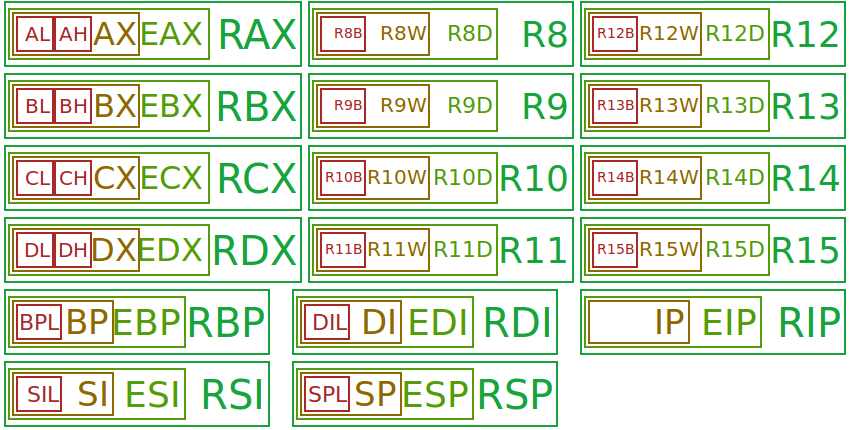
\includegraphics[width=\textwidth]{../asm/x86-gprs}
\imagecredit{Immae via Wikipedia}
\end{frame}

\begin{frame}[fragile,label=overlap]{overlapping registers (1)}
\begin{itemize}
\item setting 32-bit registers sets \myemph{whole} 64-bit register
\item extra bits are always zeroes
\end{itemize}
\begin{lstlisting}[style=small]
movq $0x123456789abcdef, %rax
    // Intel: MOVABS RAX, 0x123456789abcdef
xor %eax, %eax
// %rax is 0, not 0x1234567800000000
movl $-1, %ebx
    // Intel: MOV EBX, -1
// %rbx is 0xFFFFFFFF, not -1 (0xFFFFF...FFF)
\end{lstlisting}
\begin{itemize}
\item 32-bit instructions are often shorter than 64-bit ones, \\
so compilers will prefer \texttt{mov \$1234, \%ecx} to \texttt{mov \$1234, \%rcx}
\end{itemize}
\end{frame}

\begin{frame}[fragile,label=overlap2]{overlapping registers (2)}
\begin{itemize}
\item setting \myemph{8/16-bit registers} doesn't change rest of 64-bit register:
\end{itemize}
\begin{lstlisting}[style=small]
movq $0x12345789abcdef, %rax
movw $0xaaaa, %ax
// %rax is 0x123456789abaaaa
\end{lstlisting}
\end{frame}

